% Standalone TikZ diagram: run make in this directory for PDF and SVG.
\documentclass[11pt,tikz,border=2pt]{standalone}
% Shared typography and graph grammar for the L5a standalone TikZ diagrams.
\usepackage{fontspec}
\IfFontExistsTF{Helvetica Neue Light}{
  \setsansfont{Helvetica Neue Light}[BoldFont={Helvetica Neue Medium}]
}{\setsansfont{TeX Gyre Heros}}
\renewcommand{\familydefault}{\sfdefault}
\usepackage{amsmath,amssymb}
\usepackage{unicode-math}
\setmathfont{latinmodern-math.otf}
\usetikzlibrary{arrows.meta,calc,positioning}
\definecolor{vnslideink}{HTML}{333333}
\definecolor{vnslidebody}{HTML}{5E5E5E}
\definecolor{vnaccent}{HTML}{FF644E}
\definecolor{vnslidelink}{HTML}{579ACA}
\definecolor{vnquiet}{HTML}{899198}
\pagecolor{white}
\tikzset{
  every picture/.style={font=\sffamily\small,text=vnslidebody},
  vertex/.style={circle,draw=vnslideink,fill=white,line width=0.7pt,
    minimum size=6.4mm,inner sep=0pt,font=\sffamily\normalsize},
  edge/.style={draw=vnslidebody,line width=0.8pt,
    -{Latex[length=2.2mm,width=1.5mm]},shorten <=3.4mm,shorten >=3.4mm},
  active/.style={edge,draw=vnaccent,line width=1.2pt},
  residual/.style={edge,draw=vnslidelink,line width=1.2pt},
  inactive/.style={edge,draw=vnquiet,line width=0.7pt},
  edge label/.style={fill=white,inner sep=1.4pt,font=\sffamily\small},
  partition/.style={rounded corners=2mm,line width=0.5pt},
}

\begin{document}
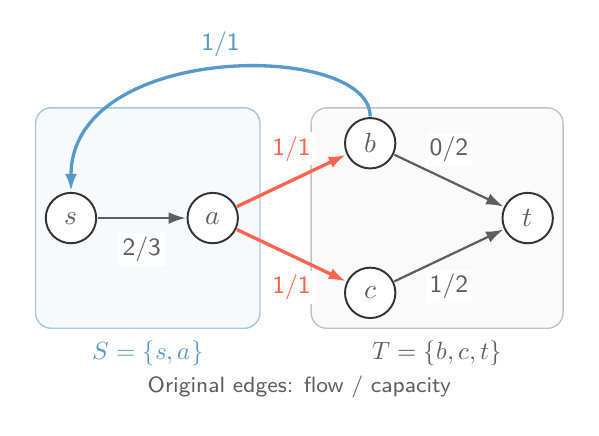
\begin{tikzpicture}[x=1cm,y=1cm]
  % S and T partition the original vertices; colored edges cross the cut.
  \draw[partition,draw=vnslidelink!55,fill=vnslidelink!5]
    (-0.45,-1.4) rectangle (2.4,1.4);
  \draw[partition,draw=vnquiet!55,fill=black!2]
    (3.05,-1.4) rectangle (6.25,1.4);
  \coordinate (s) at (0,0);
  \coordinate (a) at (1.8,0);
  \coordinate (b) at (3.8,0.95);
  \coordinate (c) at (3.8,-0.95);
  \coordinate (t) at (5.8,0);
  \draw[edge] (s)--node[edge label,below=5pt]{2/3}(a);
  \draw[active] (a)--node[edge label,above=5pt,text=vnaccent]{1/1}(b);
  \draw[active] (a)--node[edge label,below=5pt,text=vnaccent]{1/1}(c);
  \draw[edge] (b)--node[edge label,above=5pt]{0/2}(t);
  \draw[edge] (c)--node[edge label,below=5pt]{1/2}(t);
  \draw[residual] (b) .. controls (3.8,2.25) and (0,2.25) ..
    node[edge label,above=5pt,text=vnslidelink]{1/1}(s);
  \foreach \v in {s,a,b,c,t} {\node[vertex] at (\v) {$\v$};}
  \node[text=vnslidelink] at (0.98,-1.72) {$S=\{s,a\}$};
  \node at (4.65,-1.72) {$T=\{b,c,t\}$};
  \node[font=\sffamily\footnotesize] at (2.9,-2.15) {Original edges: flow / capacity};
  \path[use as bounding box] (-0.55,-2.35) rectangle (6.35,2.05);
\end{tikzpicture}
\end{document}
